\clearpage
\section{两块玻璃的颜色与折射}
打开项目面板里的 \path{Glass-Studio.redflag}，墙前立着两片玻璃。在属性中选「青色玻璃」的材质，将折射率从 1 改为 1.5。墙条在玻璃外保持原位，穿过边缘后却向旁边错开。下图保留了墙条在玻璃上方的一小段，可以直接沿同一条边看下来。

\begin{figure}[H]\centering
\begin{minipage}[t]{.48\linewidth}\centering
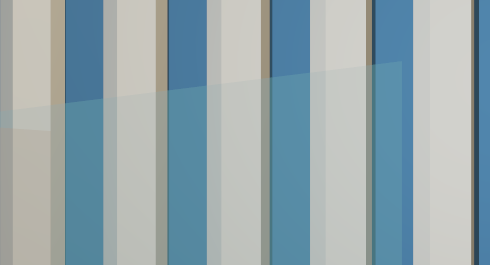
\includegraphics[width=\linewidth]{../../../output/scenes/glass-studio/straight-detail.png}\\
{\small 折射率 1.0}
\end{minipage}\hfill
\begin{minipage}[t]{.48\linewidth}\centering
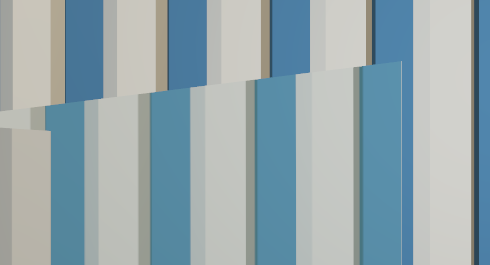
\includegraphics[width=\linewidth]{../../../output/scenes/glass-studio/bent-detail.png}\\
{\small 折射率 1.5}
\end{minipage}
\caption{演示时两块玻璃同时改动。图为 Vulkan 编辑器两次运行的第 12 帧、同一位置的裁剪。左图的墙条变了颜色，右图的墙条在边缘处还发生位移。\href{run:../scenes/glass-studio/bent.png}{完整视口图}}
\end{figure}

先看颜色。一个像素若同时落在两块玻璃上，琥珀色玻璃的不透明度是 0.30，青色是 0.24。第一层剩下 $1-0.30=0.70$ 的背景，第二层又留下其中的 $0.76$，最后约有 $53.2\%$ 的背景颜色。引擎用两个数的对数之和保存这个乘积，合成时取指数就能还原。两种玻璃各自贡献多少颜色，则按不透明度和深度加权平均。这样几何可以直接按场景中的次序提交；当颜色差异很大且紧密交叠时，这个平均值是近似。

再看墙条的位置。把玻璃面的垂直方向叫作法线，入射角和折射角均从它量起。空气的折射率近似为 1，玻璃取 1.5。斯涅尔定律给出 $1\sin\theta_i=1.5\sin\theta_t$。若入射角为 $30^\circ$，折射角约为 $19.5^\circ$，光线在玻璃中向法线靠拢。\code{CompositeTransparency.comp} 的 \code{main} 用 \code{refract} 得到这个方向，再按材质给出的世界单位厚度，求光线到达另一面的地点。把这个点投回屏幕，就知道该去墙面图的哪里读颜色。落在屏幕外时，保留原处背景；落在玻璃前方的遮挡物上，对应的采样点也沿原方向取色。

这张墙面图已经算完直接光、间接光以及开启的反射和雾。两片玻璃重叠时，合成只使用一组加权的方向和厚度，因此无法还原光线多次进出玻璃的路线。用两次回放的完整图逐点比较，在 $1{,}243{,}949$ 个像素中，$157{,}890$ 个至少有一个显示颜色通道变化超过 $8/255$。这是这个场景的画面差异；验证绘制顺序则另用两片测试网格，调换顺序后读回的最大颜色差为 0。

\readings{\src{Redflag/src/Platform/Vulkan/Shaders/Mesh.frag}{Mesh.frag · main}\quad
\src{Redflag/src/Platform/Vulkan/Shaders/CompositeTransparency.comp}{CompositeTransparency.comp · main}\quad
\href{run:../scenes/glass-studio/capture.json}{帧、事件与像素}\\
\href{https://learnopengl.com/Advanced-OpenGL/Blending}{LearnOpenGL · 透明度}\quad
\href{https://jcgt.org/published/0002/02/09/}{McGuire 与 Bavoil · 加权混合}\quad
\href{https://pbr-book.org/4ed/Reflection_Models/Specular_Reflection_and_Transmission}{PBRT 第四版 §9.3 · 折射}}
